% Created 2013-04-10 Wed 04:21
\documentclass[11pt]{article}
\usepackage[utf8]{inputenc}
\usepackage[T1]{fontenc}
\usepackage{graphicx}
\usepackage{longtable}
\usepackage{float}
\usepackage{wrapfig}
\usepackage{soul}
\usepackage{amssymb}
\usepackage{hyperref}


\title{Manual de Drupal 7}
\author{David Arroyo Menéndez}
\date{10 April 2013}

\begin{document}

\maketitle

\setcounter{tocdepth}{3}
\tableofcontents
\vspace*{1cm}

Manual desarrollado por \href{http://www.davidam.com}{David Arroyo Menéndez}.  


\section{API de Drupal}
\label{sec-1}


Una API (del inglés Application Programming Interface) es un interfaz
para comunicar componentes de un sistema de software. Para cada
componente del sistema una API maneja la comunicación entre el
componente y el núcleo. Este método hace que los cambios en el
componente se aislen de los correspondientes cambios en el núcleo, de
este modo, se reducen los esfuerzos en depuración y pruebas a los
componentes únicamente.  En general, una API establece un estándar
para tratar con operaciones de bajo nivel e introducir estabilidad y
uniformidad en el código. El ejemplo más común de una API es la API de
la base de datos, que encapsula las operaciones de la base de datos
desde el núcleo, de tal modo que el núcleo funciona sin tener en
cuenta el gestor de base de datos que el sistema usa.  Ahora se verán
unos ejemplos de cómo podemos usar la api de drupal.

\subsection{db\_query}
\label{sec-1.1}


Con db\_query es posible hacer consultas select a la base de
datos. Ahora se verán las siguientes líneas de código:


\begin{verbatim}
<?php
// Drupal 7
// Notice the place holders are now done using the same syntax as PDOs (:uid)
// Placeholders also don't need to be quoted anymore.
$uid = 1;
$result = db_query('SELECT n.nid, n.title, n.created
FROM {node} n WHERE n.uid = :uid', array(':uid' => $uid));
// Result is returned as a iterable object that returns a stdClass object on each iteration
foreach ($result as $record) {
 // Perform operations on $record->title, etc. here.
 // in this example the available data would be mapped to object properties:
 // $record->nid, $record->title, $record->created
print($record->title);
}
\end{verbatim}



Primero se fija el valor del argumento (\$uid=1). Seguidamente se
ejecuta la consulta (se hace un select a la tabla node cuyo argumento
es el uid). Y finalmente, se recorren los resultados de la consulta
imprimiendo el título del nodo.  La llamada a la API de db\_query es la
siguiente:


\begin{verbatim}
db_query($query, array $args = array(), array $options = array())
Parametros:
$query Es la sentencia de consulta lista para ejecutarse. 
$args Un array de valores para sustituir en la consulta. 
$options Un array de opciones para controlar como la consulta opera.
Valor devuelto:
DatabaseStatementInterface Un objeto sentencia ya ejecutado.
\end{verbatim}



Es posible consultar la api de db\_query, para una descripción completa
de la función y sus argumentos.

\subsection{node\_load}
\label{sec-1.2}


En general, para obtener un nodo desde un nid es más cómodo utilizar
node\_load que carga un objeto nodo desde la base de datos. Ahora se
verá un ejemplo de código:


\begin{verbatim}
$nid = 1;
$node = node_load($nid);                                 
print($node->title);
\end{verbatim}



Primero se fija el valor del argumento (\$nid=1). Seguidamente se carga
el nodo cuyo nid es \$nid en \$node. Y, finalmente, se imprime el título
del nodo o lo que se quiera.  La llamada a la API de node\_load es la
siguiente:


\begin{verbatim}
node_load($nid = NULL, $vid = NULL, $reset = FALSE) 
Carga un objeto nodo desde la base de datos.
Parámetros
$nid El ID del nodo.
$vid El ID de la revisión del nodo.
$reset Si resetear la cache node_load_multiple.
Valor devuelto
Un objeto nodo completamente poblado.
\end{verbatim}



Es posible consultar la \href{http://api.drupal.org/api/drupal/modules--node--node.module/function/node_load/7}{api de node\_load}, para una descripción
completa de la función y sus argumentos.

\subsection{user\_load}
\label{sec-1.3}


De la misma manera, que no se suele usar db\_query para cargar nodos,
tampoco lo usamos para cargar usuarios. user\_load carga un objeto
usuario de la base de datos.  Ahora se verá un ejemplo de código:


\begin{verbatim}
$uid = 1;
$account = user_load($uid);                                 
print($account->name);
\end{verbatim}



Primero se fija el valor del argumento (\$uid=1). Seguidamente se carga
el usuario cuyo uid es \$uid en la tabla users. Y, finalmente, se
imprime el nombre del usuario o lo que se necesite.  

La llamada a la API de node\_load es la siguiente:


\begin{verbatim}
user_load($uid, $reset = FALSE) 

Carga un objeto usuario Drupal tiene un objeto usuario ($user) global,
que representa el usuario logado actualmente. Para evitar confusión es
una buena idea asignar el resultado de esta función a un variable
local diferente, generalmente $account. 

Si tu quieres actuar como el usuario que estás cargando, es esencial
llamar primero a: 

<?php drupal_save_session(FALSE); ?> 

Parametros $uid Entero especificando el ID del usuario a cargar.
$reset TRUE para resetear la cache interna y cargar desde la base de
datos; FALSE (por defecto) para cargar desde la caché interna, si está
asignada.  Valor devuelto Un objeto usuario completamente cargado si
ha habido éxito en la carga, si el usuario no pudo ser cargado
devuelve FALSE.
\end{verbatim}



Es posible consultar la api de \href{http://api.drupal.org/api/drupal/modules--user--user.module/function/user_load/7}{user\_load}, para una descripción
completa de la función y sus argumentos.

\subsection{Aplicando funciones de la API a nuestro proyecto Drupal}
\label{sec-1.4}


Ahora veamos como aplicar las funciones aprendidas a nuestro proyecto
Drupal. Podemos hacerlo desde varias partes:

\begin{itemize}
\item Customfield php de views
\item Templates de nuestro tema instalado
\item Templates de módulos instalados
\item Templates que modifican views
\item Módulos nuevos
\item Desde contenidos ó bloques con el filtro php activo
\end{itemize}
La parte de nuevos módulos lo abordaremos en el próximo capítulo, pero
el resto de hacks que podemos hacer a drupal sí es interesante verlo
desde aquí.

\subsection{Views php}
\label{sec-1.5}


Para tener esta funcionalidad es necesario tener instalado el módulo
views php. Este módulo te permite insertar código php en un campo de
views. Veamos cómo con un ejemplo.  

Dada la siguiente vista:

\includegraphics[width=10em]{/home/davidam/Imágenes/drupal1.png}

Pulsamos en + en el apartado ``Fields''. Encontramos un desplegable de
categorías de fields y seleccionamos ``Global''.

\href{file://.~/Imágenes/drupal2.png}{file:\~/Imágenes/drupal2.png}

Y ahí elegimos ``Global PHP'' y pulsamos ``Agregar''. En la siguiente
pantalla encontramos un montón de opciones y vamos hasta ``Value Code''
y pulsamos en ``AVAILABLE VARIABLES'' para ver las variables que tenemos
disponibles.

Ahora es el momento de recordar user\_load y ver que la variable
disponible \$row->uid nos puede servir como valor de entrada. De este
modo, se introduce el siguiente código y se pulsa en actualizar:


\begin{verbatim}
$account = user_load($row->uid);
return $account->name;
\end{verbatim}



Luego es necesario salvar la vista, teniendo un display de página ó de
bloque.

Este ejemplo podría (y debe) ser fácilmente implementado usando
views. Pero ilustra muy bien el poder de views php. Una necesidad real
donde usar views php podría ser lo siguiente:


\begin{verbatim}
global $user;
if ($user->uid == $row->uid)
{
print '[buttons]';
}
\end{verbatim}



Este código imprime algo específico (por ejemplo, botones) cuando el
usuario logado coincide con el usuario de la fila de nuestra vista.

\subsection{Templates de nuestro tema instalado}
\label{sec-1.6}


Otra situación en la que se puede querer aplicar nuestros
conocimientos de la API. Es modificando algún template del tema que
está activo ó que se ha desarrollado para el proyecto actual.

Es posible que por alguna razón un cliente pida que después del
contenido de un nodo aparezca el nombre del administrador del sitio
(cuyo uid es 1). En el caso de que el tema activo fuera barlik
abriríamos el siguiente fichero:
``themes/bartik/templates/node.tpl.php'' y debajo de print
render(\$content); se introducirían las líneas de código relativas a la
función user\_load que ya hemos visto. Quedando todo del siguiente
modo:


\begin{verbatim}
...
  <div class="content clearfix"<?php print $content_attributes; ?>>                                                           
    <?php                                                                                                                     
      // We hide the comments and links now so that we can render them later.                                                 
      hide($content['comments']);                                                                                             
      hide($content['links']);                                                                                                
      print render($content);                                                                                                 
    ?>                                                                                                                        
    <?php                                                                                                                     
$uid = 1;                                                                                                                     
$account = user_load($uid);                                                                                                   
print($account->name);                                                                                                        
    ?>                                                                                                                        
  </div>                                                                                                                      
                                                                                                                              
  <?php     
...
\end{verbatim}



\subsection{Templates de módulos instalados}
\label{sec-1.7}


Modificar templates de módulos instalados es similar a lo visto en el
anterior apartado. Tan solo es necesario localizar el template del
módulo que se pretende modificar, copiarlo en la carpeta del tema y
hacer allí las modificaciones pertinentes.

\subsection{Templates que modifican views}
\label{sec-1.8}


Si desde una vista se pulsa a Style settings -> Theme se ven los
diferentes nombres con los que es posible reescribir las plantillas
relacionadas con views. Una vez elegida la plantilla a reescribir, se
introduce el fichero en la carpeta del tema.

Ahora que ya se sabe donde aplicar la api, se puede seguir aprendiendo
nuevas funciones.

\subsection{drupal\_set\_message}
\label{sec-1.9}


Imprime un mensaje, normalmente con la acción que se acaba de
realizar. Un ejemplo:


\begin{verbatim}
<?php
drupal_set_message('Aprendiendo a usar drupal_set_message');
?>
\end{verbatim}



Este código hace aparecer la frase ``Aprendiendo a usar
drupal\_set\_message'' formateado como mensaje drupal, normalmente dentro
de una caja verde.

La llamada a la API de drupal\_set\_message es la siguiente:


\begin{verbatim}
drupal_set_message($message = NULL, $type = 'status', $repeat = TRUE)
Parámetros
$message El mensaje empieza con una mayúscula y finaliza con un punto.
$type El tipo de mensaje. Uno de los siguientes valores es posible:
+ 'status' 
+ 'warning' 
+ 'error' 
$repeat Si esto es FALSE y el mensaje ha sido asignado, entonces el mensaje no será repetido.
\end{verbatim}



Es posible consultar la \hyperref[api.drupal.org/api/drupal/includes--bootstrap.inc/function/drupal_set_message/7]{drupal\_set\_message}, para una descripción
completa de la función y sus argumentos.

\subsection{node\_save}
\label{sec-1.10}


Graba un objeto nodo en la base de datos ó añade un nuevo nodo. Ahora
se verá un ejemplo de código:


\begin{verbatim}
<?php
$node = node_load(1); // load node
$node->title = 'nah, nah, nah, nah, boo, boo'; // Do some changes
node_save($node); // save your changes
drupal_set_message('Updated');
?>
\end{verbatim}



En el ejemplo se puebla un objeto nodo cuyo nid es 1. Se establece un
título cualquiera. Se guarda el nodo modificado en la base de datos. Y
finalmente se imprime el mensaje ``Updated''.

La llamada a la API de node\_save es la siguiente:


\begin{verbatim}
node_save($node) 

Parámetros $node El objeto $node que va a ser guardado. Si $node->nid
es omitido (o $node->is_new es TRUE), un nuevo nodo será añadido.
\end{verbatim}



Es posible consultar la \href{http://api.drupal.org/api/drupal/modules--node--node.module/function/node_save/7}{api de node\_save} para una descripción
completa de la función y sus argumentos.

\subsection{user\_save}
\label{sec-1.11}


De la misma manera que escribimos las modificaciones a un nodo en base
de datos, es posible escribir en base de datos las modificaciones a un
usuario. Se presentan un par de ejemplos:


\begin{verbatim}
<?php
$account = user_load(1); // load node
user_save($account, array('name' => 'John Smith')); // save your changes
drupal_set_message('Updated');
?>
\end{verbatim}



Este ejemplo es bastante similar al de node$_{\mathrm{save}}$: tras cargar el
usuario, las modificaciones se realizan al nombre del usuario y se
salvan los datos. Ahora el siguiente ejemplo:


\begin{verbatim}
<?php
$details = array(
 'name' => 'John Smith',
 'pass' => 'sssh es un secreto',
 'mail' => 'john@smith.com',
 'access' => 0, /* optional, i didnt want user to be able to this this account yet*/
 'status' => 1
;
$user = user_save(null, $details);
?>
\end{verbatim}



En este ejemplo se usa user$_{\mathrm{save}}$ para crear usuarios nuevos, que es
otro de los usos de esta función, los valores se definen en el array
\$details.

La llamada a la API de user$_{\mathrm{save}}$ es la siguiente:


\begin{verbatim}
user_save($account, $edit = array(), $category = 'account') 
Parámetros
$account (opcional) El objeto de usuario para modificar ó añadir. Si se desea modificar una cuenta de usuario existente, se necesitará asegurar que (a) $account es un objeto, y (b) se ha asignado $account->uid al user ID de la cuenta de usuario a modificar. Si se desea crear una nueva cuenta de usuario, es posible establecer $account->is_new a TRUE u omitir el campo $account->uid.
$edit Un array de campos y valores a guardar. Por ejemplo, array('name' => 'My name'). Pares clave / valor añadidas a $edit['data'] serán serializadas y guardadas en la columna {users.data}.
$category (optional) The category for storing profile information in.
Valor devuelto
Un objeto $user si hay éxito y FALSE en caso contrario.
\end{verbatim}



Es posible consultar la \href{http://api.drupal.org/api/drupal/modules--user--user.module/function/user_save}{api de user\_save}, para una descripción
completa de la función y sus argumentos.

\subsection{watchdog}
\label{sec-1.12}


Hace un log de un mensaje de sistema. Ahora se verá un ejemplo de código:


\begin{verbatim}
<?php
function node_save_action($node) {
  node_save($node);
  watchdog('action', 'Saved @type %title', array('@type' => node_type_get_name($node), '%title' => $node->title));
}
?>
\end{verbatim}



Antes de explicar el código veamos la declaración de la API:


\begin{verbatim}
watchdog($type, $message, $variables = array(), $severity = WATCHDOG_NOTICE, $link = NULL) 
Parámetros
$type La categoría al que el mensaje pertenece. Puede ser cualquier cadena, pero la práctica general es usar el nombre del módulo llamando watchdog().
$message El mensaje a almacenar en el log. ¡Deja el $message traducible no concatenando valores dinámicos dentro de él! 
$variables Array de variables para reemplazar en el mensaje ó NULL si el mensaje ya está traducido ó no es posible traducirlo
$severity La gravedad del mensaje, dada en el RFC 3164. Posibles valores son WATCHDOG_ERROR, WATCHDOG_WARNING, etc.
$link Un enlace asociado con el mensaje.
\end{verbatim}



En nuestro ejemplo \$type es ``action'', \$message es ``Saved @type
\%tittle'' y las variables type y title se obtienen mediante el array.

Es posible consultar la api de watchdog, para una descripción completa
de la función y sus argumentos.

\subsection{t}
\label{sec-1.13}


La función t facilita la traducción de cadenas en Drupal. Ahora se
verá un ejemplo de código:


\begin{verbatim}
<?php
print(t('Hello World'));
?>
\end{verbatim}



Este código imprime la cadena ``Hello world''. Pero ahora la cadena
``Hello world'' es traducible. Si se va a Configuración -> Regional e
Idioma -> Traducir Interfaz -> Traducir podemos buscar la cadena
``Hello world'' y traducirla por ``Hola Mundo'' en español.

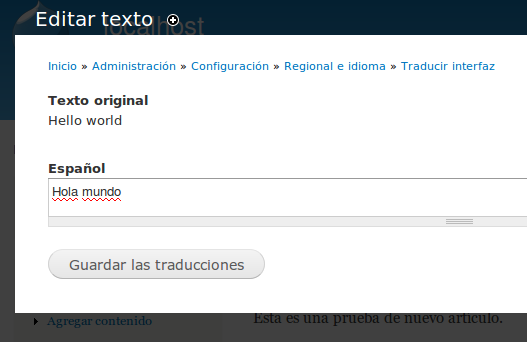
\includegraphics[width=10em]{/home/davidam/public_html/docu/drupal/pantallazo4.png}

Ahora se verá otro ejemplo:


\begin{verbatim}
$uid = 1;
$account = user_load($uid);
print(t("@name's blog", array('@name' => format_username($account))));
\end{verbatim}



Como se ve es posible introducir variables en la cadena a traducir que
son definidas en el segundo argumento de t que es un array.  

La llamada a la API de t es la siguiente:


\begin{verbatim}
t($string, array $args = array(), array $options = array())
\end{verbatim}



Es posible consultar la \href{http://api.drupal.org/api/drupal/includes--bootstrap.inc/function/t/7}{api de t}, para una descripción completa de la
función y sus argumentos.

\subsection{db\_insert}
\label{sec-1.14}


Esta función permite insertar registros en la base de datos. Ahora se
verá un ejemplo:


\begin{verbatim}
<?php
$nid = db_insert('node') // Table name no longer needs {}
->fields(array(
'title' => 'Example','uid' => 1, 'created' => REQUEST_TIME,
))->execute();
\end{verbatim}



El código inserta un nuevo registro en la tabla node, con los
parámetros dados. Como se vé este código es alternativo a utilizar
node$_{\mathrm{save}}$. Ahora se verá la descripción de la llamada a la API.


\begin{verbatim}
db_insert($table, array $options = array()) 
Devuelve un nuevo objeto InsertQuery para la base de datos activa.
Parametros
$table La tabla en la que se hace la inserción
$options Un array de opciones para controlar cómo opera la consulta.
Valor devuelto
InsertQuery Un nuevo objeto InsertQuery para esta conexión.
\end{verbatim}



Es posible consultar la api de \href{http://api.drupal.org/api/drupal/includes--database--database.inc/function/db_insert/7}{db\_insert}, para una descripción
actualizada de la función y sus argumentos.

\subsection{db\_update}
\label{sec-1.15}


Actualiza registros de la base de datos. Ahora un ejemplo:


\begin{verbatim}
<?php
$num_updated = db_update('node') // Table name no longer needs {}
->fields(array(
 'uid'=>5,
 'status'=>1,
))
->condition('created',REQUEST_TIME-3600,'>=')
->execute();
?>
\end{verbatim}



Este ejemplo ejecuta la siguiente consulta SQL: 


\begin{verbatim}
UPDATE {node} SET uid=5, status=1 WHERE created >= 1221717405"
\end{verbatim}



La llamada a la API de db$_{\mathrm{update}}$ es la siguiente:


\begin{verbatim}
db_update($table, array $options = array()) 
Devuelve un nuevo objeto UpdateQuery para la base de datos activa.
Parámetros
$table La tabla a actualizar.
$options Un array de opciones para controlar cómo opera la consulta.
Valor devuelto
UpdateQuery Un nuevo objeto UpdateQuery para esta conexión.
\end{verbatim}



Es posible consultar la \href{http://api.drupal.org/api/drupal/includes--database--database.inc/function/db_update/7}{api de db\_update}, para una descripción
actualizada de la función y sus argumentos.

\subsection{db\_delete}
\label{sec-1.16}


Elimina registros de la base de datos. Ahora un ejemplo:


\begin{verbatim}
<?php
$nid=5;                             
$num_deleted=db_delete('node')->condition('nid',$nid)->execute();
?>
\end{verbatim}



Este ejemplo es equivalente a la consulta SQL ``DELETE FROM \{node\}
WHERE nid = 5''.

La llamada a la API de db$_{\mathrm{delete}}$ es la siguiente:


\begin{verbatim}
db_delete($table, array $options = array()) 
Devuelve un nuevo objeto DeleteQuery para la base de datos activa.
Parámetros
$table La tabla dónde se suprimen las filas
$options Un array de opciones para controlar cómo la consulta opera.
Valor devuelto
DeleteQuery Un nuevo objeto DeleteQuery para esta conexión.
\end{verbatim}



Es posible consultar la \href{http://api.drupal.org/api/drupal/includes--database--database.inc/function/db_delete/7}{api de db\_delete}, para una descripción
actualizada de la función y sus argumentos.

\section{Desarrollo de Módulos}
\label{sec-2}


\subsection{Arquitectura de los Módulos de Drupal}
\label{sec-2.1}


¿Qué es exactamente un módulo y cuál es su propósito?

La segunda pregunta es fácil de responder: un módulo Drupal es un
mecanismo diseñado para proporcionar un método uniforme de extender
las funcionalidades de Drupal. Esta respuesta nos acerca bastante a
responder a la primera cuestión. Un módulo es un conjunto de código
PHP y ficheros que usan la API de Drupal y la arquitectura para
integrar nuevos componentes funcionales dentro del framework
Drupal. Un propósito de este manual es explicar cómo escribir este
código.
 
Empecemos ahora a echar un vistazo a la arquitectura del módulo. Los
ficheros que crean los módulos están agrupado dentro de localizaciones
específicicas bajo la estructura de directorios de Drupal. Esto es, en
el sistema de fichero de la instalación de Drupal, los módulos Drupal
deben residir en unos pocos lugares. 

Cuando Drupal necesita información acerca de sus módulos, mirará en
estos lugares predeterminados. Cada módulo está contenido en su propio
directorio, y tiene al menos 2 ficheros—uno describiendo el contenido
del módulo y uno ó más ficheros conteniendo código y otro material de
soporte.  

Antes de que un módulo pueda ser usado, debe ser activado por un
administrador de Drupal. Sin embargo, una vez un módulo es activado,
entonces es cargado cuando se le requiere y Drupal pasa las
solicitudes al módulo.

\subsection{Módulos del Núcleo}
\label{sec-2.2}


Algunos módulos son tan importantes que eliminándolos desactivarías
funcionalidades esenciales para el funcionamiento de Drupal. También,
hay módulos que proporcionan funcionalidades necesarias por una amplia
variedad de sistemas. Estos dos grupos de módulos, son mantenidos por
el equipo de desarrolladores de Drupal, y son colectivamente referidos
como los Módulos del Núcleo de Drupal. Estos módulos están incluidos
por defecto en la instalación de Drupal, y tienen un activo
mantenimiento y desarrollo por la comunidad Drupal.

A pesar de este importante rol, hay pocas distinciones entre los
Módulos del Núcleo de Drupal y cualquier otro módulo. Ellos siguen las
mismas directrices y usan la misma API. No hay nada particularmente
arcano en estos módulos.

Desde la sección de administración de Drupal, es posible ver la lista
de los módulos del núcleo en Administración -> Módulos.

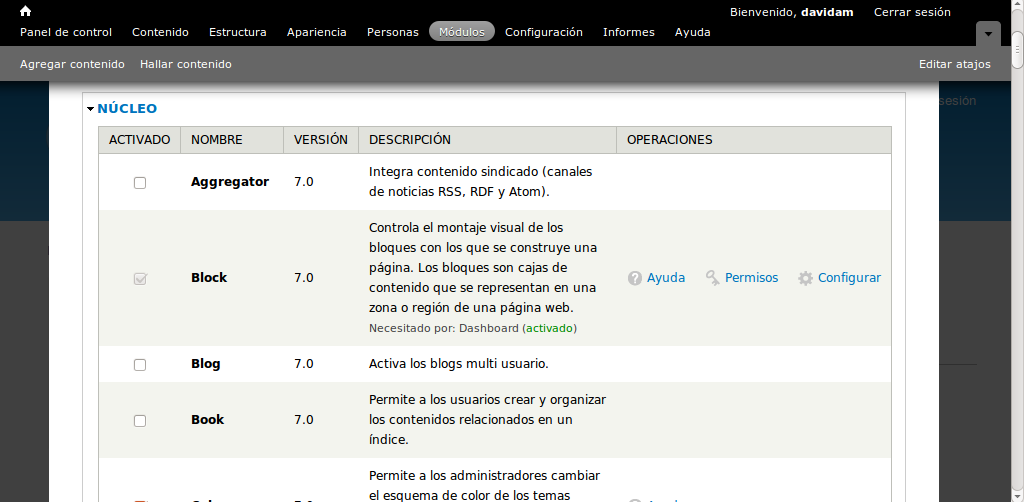
\includegraphics[width=10em]{/home/davidam/public_html/docu/drupal/pantallazo5.png}

Una de las maravillas de la arquitectura de Drupal es la facilidad con
que varios módulos interactúan. Usando la arquitectura de hook, los
servicios que los módulos proporcionan pueden ser tejidos juntos para
crear robustas funcionalidades sin copiosas cantidades de código.

Los módulos del core proporcionan una excelente referencia para saber
cómo el código de Drupal debe ser escrito.

\subsection{Hooks}
\label{sec-2.3}


¿Cómo Drupal sabe cuando invocar a un módulo para manejar una
solicitud particular?. Esto es hecho a través del mecanismo de hooks,
que nosotros examinaremos cuidadosamente en este manual. Para empezar,
una breve explicación de cómo funcionan los hooks. Cuando Drupal
gestiona una solicitud desde un usuario, procede a través de una serie
de pasos. Por ejemplo, el núcleo de Drupal primero inicia la
aplicación, definiendo variables críticas y funciones frecuentemente
usadas. Lo siguiente es, cargar librerías críticas, temas y
módulos. Lo siguiente es, continuar procesando la solicitud, mapeando
la URI solicitada al código que la maneja y así. Después, aplica un
tema a los datos, formateando información como salida. Finalmente,
devuelve la salida al navegador del usuario.

En este paso a paso, hay momentos predefinidos en los que Drupal
ejecuta hooks. ¿Qué significa esto?. En resumen, significa que Drupal
examina algunos ó todos los módulos actualmente activados que siguen
específicos y predefinidos patrones. Algunos tienen enlazado a este
proceso un método ``callback''.

Por ejemplo, mientras se está creando el contenido para una página
vista, Drupal podría escanear módulos para funciones llamadas
<modulename>\_block() y <modulename>\_view() (donde <modulename> es
reemplazado por el nombre de cada módulo que chequea).

Los módulos que contienen tales funciones son aquellos que implementan
hook\_block() y hook\_view().

Cuando Drupal encuentra tales funciones, las ejecuta, y usa los datos
de estas funciones para devolver una respuesta que enviar al
usuario. Drupal continúa su procesamiento de la solicitud paso por
paso, quizás ejecutando muchos otros hooks. Una vez que todos los
pasos han sido completados y una respuesta ha sido enviada al usuario,
Drupal se limpia a sí mismo y termina la ejecución.

Los módulos pueden definir sus propios hooks, que otros módulos pueden
usar. De este modo, el mecanismo de hook puede ser extendido para
proporcionar un personalizado comportamiento complejo.

Cuando un módulo proporciona una función que empareja una firma hook,
nosotros decimos que este módulo implementa este hook. Por ejemplo,
imagina que Drupal tiene hook llamado hook\_example. Si nosotros
definiéramos un módulo llamado mimodulo que contuviera una función
llamada mimodulo\_example(), estaríamos implementando hook\_example().

\subsection{Creación de Bloques}
\label{sec-2.4}


Esta sección tiene un doble objetivo: introducir a la api de bloques y
crear un primer módulo. Y en el siguiente capítulo se verá cómo
instalar dicho módulo.

En Drupal, cada módulo está contenido en su propio directorio. Esto
simplifica la organización; todos los ficheros de un módulo están
localizados en un lugar. Así que vamos a crear un directorio que sea
descriptivo del bloque que vamos a crear en nuestro caso mibloque.


\begin{verbatim}
cd sites/all/modules
mkdir mibloque
\end{verbatim}



Una vez se ha creado el directorio, es posible empezar a crear
ficheros para el módulo. El primer fichero a crear será el fichero
.info.

\subsection{Creando un fichero .info}
\label{sec-2.5}

El fichero .info es escrito como un fichero PHP INI, que es un formato
para configuraciones simples.

El fichero .info debe seguir las convenciones de nombres estándar para
módulos. Debe ser nombrado <modulename>.info, donde <modulename> es el
mismo que el nombre del directorio. Nuestro fichero, por tanto, será
llamado mibloque.info.

Lo siguiente son los contenidos de mibloque.info:


\begin{verbatim}
;$Id$ 
name = "Mi Bloque" 
description = "Muestra un bloque creado desde la API" 
core = 7.x
\end{verbatim}



Este fichero no es particularmente grande. La primera línea del
fichero es, a primera vista, la más críptica. Sin emabargo, su función
es mundana: es la variable para servidor CVS o Subversion de Drupal.

Las siguientes 3 directivas proporcionan información del módulo a
Drupal.

La directiva name proporciona un nombre “legible por humanos” para el
módulo. Anteriormente, ya se ha visto brevemente cómo se activa un
módulo. Los nombres de los módulos que se vieron se extrajeron de la
directiva name de los ficheros .info. Aquí hay un ejemplo:

\href{file:///home/davidam/public_html/docu/drupal/pantallazo8.png}{file:\~/public\_html/docu/drupal/pantallazo8.png}  

En el pantallazo los nombres ``Aggregator'' y ``Block'' son tomado de las
directivas name de sus respectivos fichero .info.

Otra directiva que también aparece en el pantallazo es description
(``Descripción'').

La tercera directiva es core. Esta directiva especifica que versión de
Drupal es requerida para que el módulo funcione de manera
apropiada. El valor 7.x indica que el módulo funcionará en Drupal
(incluidas sus revisiones). En muchos casos, el empaquetador de Drupal
será capaz de establecer esto correctamente de manera automática. Pero
los desarrolladores de Drupal sugieren que esta directiva sea asignada
manualmente para quienes trabajan desde CVS.

\subsection{Un fichero .module}
\label{sec-2.6}


Como mencionamos en el primer capítulo, hay dos ficheros que cualquier
módulo debe tener (aunque muchos módulos tienen más). El primero, es
el fichero .info, del que ya se ha hablado. El segundo fichero es el
fichero .module, que es un fichero script en PHP. Este fichero
implementa un puñado de funciones hook que Drupal llamará en
predeterminadas veces durante una solicitud.

Aquí, se creará un fichero .module que mostrará uns pequeña y
formateada sección de información. Después en este capítulo, se
configurará Drupal para mostrar esto a los visitantes del sitio.

\subsection{Nuestro objetivo: Dos Block Hook}
\label{sec-2.7}


Para este muy primer módulo, se implementará las funciones
hook\_block\_info() y hook\_block\_view(). En dialecto Drupal, un bloque
es un trozo de información auxiliar que es mostrada en una página a lo
largo de la página principal de contenido. ¿Suena confuso? Un ejemplo
podría ayudar. Piensa en tu sitio web favorito de noticias. En una
típica página de artículo, el texto del artículo es mostrado en la
mitad de la página. Pero en los laterales y quizás arriba y abajo, hay
otros trozos de información: un menú del sitio, una lista de enlaces a
artículos relacionados, enlaces a comentarios ó foros acerca del
artículo, etc. En Drupal, estas piezas extra son tratadas como
bloques.

\subsection{Empezando el .module}
\label{sec-2.8}


Como ya se mencionó, Drupal sigue una codificación rigurosa y
estándares de documentación (\href{http://drupal.org/coding-standards}{http://drupal.org/coding-standards}). En
este manual, se hará todo lo posible por seguir estos estándares. Así
que al empezar el módulo, la primera cosa que se hace es proporcionar
alguna documentación para el API.

Empecemos con nuestro fichero  mibloque.module.


\begin{verbatim}
<?php 
// $Id$ 
/** 
 @file 
 Module for show data in a block
 This module provides block content builded from the api
*/
\end{verbatim}



Después del PHP tag ``<?php'' encontramos la palabra clave para el
control de versiones: 

// $Id$ 

Cuando el módulo sea chequeado dentro del Drupal CVS, la información
acerca de la actual revisión es fijada ahí.  

La tercera parte de este ejemplo es la documentación del API. Esta
documentación es contenido en un bloque de comentario especial, que
comienza con \emph{** y finaliza con *}. Cualquier cosa entre esto es
tratada como documentación. Programas de extracción como Doxygen
pueden extraer esta información y crear información de programación
útil para el usuario final.

\subsection{La implementación de hook\_block\_info()}
\label{sec-2.9}


El módulo muestra información dentro de un bloque Drupal. Para hacer
esto, nosotros necesitamos implementar las funciones hook$_{\mathrm{block}}$$_{\mathrm{info}}$()
y hook\_block\_view(). La primera nos da la información de configuración
de bloque y la segunda define lo que va a ser visto en el bloque.

Todos los métodos hook siguen la convención de nombre: <module
name>\_<hook name>. Así nuestro hook de bloque se llamará
mibloque\_block\_info().


\begin{verbatim}
/** 
\section{Implementation of hook_block_info()}
\label{sec-3}

*/

function mibloque_block_info() { 
  $blocks = array(); 

  $blocks['info'] = array( 
    'info' => t('My block') 
  ); 

  return $blocks; 
}
\end{verbatim}



En este ejemplo solo vamos a darle un valor a la cadena con la que
identificaremos nuestro bloque en la administración de bloques.

\subsection{La implementación de hook\_block\_view()}
\label{sec-3.1}


Ahora veamos como establecer un título y un cuerpo para nuestro bloque:


\begin{verbatim}
/** 
\section{Implementation of hook_block_view()}
\label{sec-4}

*/ 

function mibloque_block_view($delta = ''){ 
  $block = array(); 
 $block['subject'] = t('Título de Mi Bloque'); 
  $block['content'] = t('Cuerpo de Mi Bloque'); 
 return $block; 
}
\end{verbatim}



Como se ve es bastante similar que en el hook anterior se establece un
array al que le vamos metiendo los valores a introducir.

\subsection{Instalación de Módulos}
\label{sec-4.1}


Para poder visualizar el resultado del módulo escrito es necesario
aprender a instalar módulos. En Drupal 7 es posible instalar módulos
desde el ``Update Manager'' (navegar a Administración -> Módulos y allí
hacer click a ``Instalar nuevo módulo''). De este modo, introducimos la
url del módulo a instalar y todo se hace automáticamente. En nuestro
caso, tenemos el módulo en local, así es que debemos instalar nuestro
módulo al viejo estilo.

El directorio de nuestro módulo debe estar en el directorio
drupal/sites/all/modules, fijaos que también existe drupal/modules
pero en ese directorio solo deben estar los módulos del núcleo de
Drupal. En caso de que no esté lo copiamos:


\begin{verbatim}
cp -r mibloque /var/www/drupal/sites/all/modules
\end{verbatim}



Ahora ya podemos ir a Administración -> Módulos y buscar nuestro
módulo. Lo activamos y pulsamos guardar configuración.

Lo siguiente es activar el bloque desde Administración -> Estructura
-> Bloques y ya se puede ver el resultado:


\includegraphics[width=10em]{/home/davidam/public_html/docu/drupal/pantallazo10.png}

\subsection{Form API}
\label{sec-4.2}


Ahora un tutorial paso a paso para aprender la api de
formularios. Este tutorial es una traducción y adaptación de
\href{http://drupal.org/node/262422}{http://drupal.org/node/262422}.

Lo primero es crear un módulo dónde vamos a ir introduciendo el código
para ejecutar la api form. Seguid el paso a paso para aprender a
visualizar los ejemplos:

\begin{enumerate}
\item Crear un nuevo directorio en sites/all/modules y llamarlo `form\_tutorial'.
\item Crear un fichero llamado form\_tutorial.info en el directorio
   form\_tutorial con los siguientes contenidos:
\end{enumerate}
\begin{verbatim}
name = Form tutorial
description = Module for form api tutorial
core = 7.x
\end{verbatim}


\begin{enumerate}
\item Crear un fichero y llamarlo form\_tutorial.module. Cortar y pegar
   el primer ejemplo de código dentro de form\_tutorial.module (indicar
   que es preferible omitir el tag de cierre ?>).
\item Activar “Form tutorial” en admin/modules.
\item Escribir lo siguiente en la barra de direcciones del navegador:
   \href{http://yoursite_site_url/?q=form_tutorial/form}{http://yoursite\_site\_url/?q=form\_tutorial/form} ó
   \href{http://yoursite_site_url/form_tutorial/form}{http://yoursite\_site\_url/form\_tutorial/form} dependiendo de su
   configuración.
\item Para cada ejemplo de código en el tutorial, reemplazar el código
   de la función form\_tutorial\_my\_form en form\_tutorial.module con el
   nuevo trozo de código y escribir lo siguiente en la barra de
   direcciones del navegador:
   \href{http://yoursite_site_url/?q=form_tutorial/form}{http://yoursite\_site\_url/?q=form\_tutorial/form} ó
   \href{http://yoursite_site_url/form_tutorial/form}{http://yoursite\_site\_url/form\_tutorial/form} dependiendo de su
   configuración.
\end{enumerate}
\subsection{Formulario Básico}
\label{sec-4.3}


Este es un formulario muy básico que será extendido en los siguientes
ejemplos.


\begin{verbatim}
<?php

// This function defines the URL to the page created etc.
// See http://api.drupal.org/api/function/hook_menu/6
function form_tutorial_menu() {
 $items = array();
 $items['form_tutorial/form'] = array(
 'title' => t('My form'),
 'page callback' => 'form_tutorial_form',
 'access arguments' => array('access content'),
 'description' => t('My form'),
 'type' => MENU_CALLBACK,
 );
 return $items;
}

// This function gets called in the browser address bar for: 
//"http://yourhost/form_tutorial/form" or 
//"http://yourhost/?q=form_tutorial/form". It will generate// a page with //this form on it.

function form_tutorial_form() {

 // This form calls the form builder function via the
 // drupal_get_form() function which takes the name of this form builder
 // function as an argument. It returns the results to display the form. 
return drupal_get_form('form_tutorial_my_form');

}

// This function is called the "form builder". It builds the form.
// Notice, it takes one argument, the $form_state
function form_tutorial_my_form($form_state) {
 
 // This is the first form element. It's a textfield with a label, "Name"
 $form['name'] = array(
 '#type' => 'textfield',
 '#title' => t('Name'),
 );
 return $form;
}
?>
\end{verbatim}



La primera función implementa hook$_{\mathrm{menu}}$ y dicho de manera muy somera
nos da el acceso url desde el que visualizaremos la página que
implementa el formulario.

form$_{\mathrm{tutorial}}$$_{\mathrm{menu}}$ tiene un callback a nuestra segunda función
form$_{\mathrm{tutorial}}$$_{\mathrm{form}}$, por lo que el contenido de la página que hemos
creado será lo que devuelva form$_{\mathrm{tutorial}}$$_{\mathrm{form}}$. Esto es el resultado
de drupal$_{\mathrm{get}}$$_{\mathrm{form}}$ habiendo pasado como argumento el array definido en
form$_{\mathrm{tutorial}}$$_{\mathrm{my}}$$_{\mathrm{form}}$ que simplemente tiene el título `Name'.

\subsection{Formulario Básico con Botón Submit}
\label{sec-4.4}


Ahora se añade un botón submit al formulario anterior.


\begin{verbatim}
<?php

function form_tutorial_my_form($form_state) {
 $form['description'] = array(
 '#type' => 'item',
 '#title' => t('A simple form with a submit button'),
 );
 
 $form['name'] = array(
 '#type' => 'textfield',
 '#title' => t('Name'),
 );
 $form['submit'] = array(
 '#type' => 'submit',
 '#title' => t('Submit'),
 );
 return $form;
}
?>
\end{verbatim}



En este ejemplo tan solo hemos añadido una descripción y el botón
submit.

\subsection{Un formulario básico con fieldset}
\label{sec-4.5}


Ahora se verá cómo añadir fieldset (conjunto de campos).


\begin{verbatim}
<?php
function form_example_tutorial_3($form, &$form_state) {
  $form['description'] = array(
    '#type' => 'item', 
    '#title' => t('A form with a fieldset'),
  );

  $form['name'] = array(
    '#type' => 'fieldset', 
    '#title' => t('Name'),
  );
  $form['name']['first'] = array(
    '#type' => 'textfield', 
    '#title' => t('First name'),
  );
  $form['name']['last'] = array(
    '#type' => 'textfield', 
    '#title' => t('Last name'),
  );


  $form['submit'] = array(
    '#type' => 'submit', 
    '#value' => 'Submit',
  );
  return $form;
}
?>
\end{verbatim}



\subsection{Formulario Básico con Campos Obligatorios}
\label{sec-4.6}



\begin{verbatim}
<?php
function form_example_tutorial_4($form, &$form_state) {
  $form['description'] = array(
    '#type' => 'item', 
    '#title' => t('A form with validation'),
  );

  $form['name'] = array(
    '#type' => 'fieldset', 
    '#title' => t('Name'),
    // Make the fieldset collapsible. 
    '#collapsible' => TRUE, // Added 
    '#collapsed' => FALSE, // Added
  );

  // Make these fields required.
  $form['name']['first'] = array(
    '#type' => 'textfield', 
    '#title' => t('First name'), 
    '#required' => TRUE, // Added
  );
  $form['name']['last'] = array(
    '#type' => 'textfield', 
    '#title' => t('Last name'), 
    '#required' => TRUE, // Added
  );

  $form['submit'] = array(
    '#type' => 'submit', 
    '#value' => 'Submit',
  );
  return $form;
}
?>
\end{verbatim}



\subsection{Formulario Básico con Atributos de Elementos Adicionales}
\label{sec-4.7}



\begin{verbatim}
<?php
function form_example_tutorial_5($form, &$form_state) {
  $form['description'] = array(
    '#type' => 'item', 
    '#title' => t('A form with additional attributes'), 
    '#description' => t('This one adds #default_value and #description'),
  );
  $form['name'] = array(
    '#type' => 'fieldset', 
    '#title' => t('Name'), 
    '#collapsible' => TRUE, 
    '#collapsed' => FALSE,
  );

  $form['name']['first'] = array(
    '#type' => 'textfield', 
    '#title' => t('First name'), 
    '#required' => TRUE, 
    '#default_value' => "First name", // added default value. 
    '#description' => "Please enter your first name.", // added description 
    '#size' => 20, // added 
    '#maxlength' => 20, // added
  );
  $form['name']['last'] = array(
    '#type' => 'textfield', 
    '#title' => t('Last name'), 
    '#required' => TRUE,
  );
  $form['submit'] = array(
    '#type' => 'submit', 
    '#value' => 'Submit',
  );
  return $form;
}
?>
\end{verbatim}



\subsection{Formulario Básico con Manejador de la Validación}
\label{sec-4.8}


Ahora se va a introducir un campo fecha en el que solo podamos
introducir valores entre 1900 y el 2000.


\begin{verbatim}
function form_example_tutorial_6($form, &$form_state) {
  $form['description'] = array(
    '#type' => 'item',
    '#title' => t('A form with a validation handler'),
  );

  $form['name'] = array(
    '#type' => 'fieldset',
    '#title' => t('Name'),
    '#collapsible' => TRUE,
    '#collapsed' => FALSE,
  );
  $form['name']['first'] = array(
    '#type' => 'textfield',
    '#title' => t('First name'),
    '#required' => TRUE,
    '#default_value' => "First name",
    '#description' => "Please enter your first name.",
    '#size' => 20,
    '#maxlength' => 20,
  );
  $form['name']['last'] = array(
    '#type' => 'textfield',
    '#title' => t('Last name'),
    '#required' => TRUE,
  );

  // New form field added to permit entry of year of birth.
  // The data entered into this field will be validated with
  // the default validation function.
  $form['year_of_birth'] = array(
    '#type' => 'textfield',
    '#title' => "Year of birth",
    '#description' => 'Format is "YYYY"',
  );

  $form['submit'] = array(
    '#type' => 'submit',
    '#value' => 'Submit',
  );
  return $form;
}



/**
 * Now we add a handler/function to validate the data entered into the
 * "year of birth" field to make sure it's between the values of 1900
 * and 2000. If not, it displays an error. The value report is
 * $form_state['values'] (see http://drupal.org/node/144132#form-state).
 *
 * Notice the name of the function. It is simply the name of the form
 * followed by '_validate'. This is always the name of the default validation
 * function. An alternate list of validation functions could have been provided
 * in $form['#validate'].
 *
 * @see form_example_tutorial_6()
 *
 */
function form_example_tutorial_6_validate($form, &$form_state) {
  $year_of_birth = $form_state['values']['year_of_birth'];
  if ($year_of_birth && ($year_of_birth < 1900 || $year_of_birth > 2000)) {
    form_set_error('year_of_birth', 'Enter a year between 1900 and 2000.');
  }
}
\end{verbatim}



Como se ahora aparece al final del código una nueva función
(form$_{\mathrm{example}}$$_{\mathrm{tutorial}}$$_6$$_{\mathrm{validate}}$) que es la que hace la validación.

\subsection{Formulario con un manejador de submit}
\label{sec-4.9}



\begin{verbatim}
function form_example_tutorial_7($form, &$form_state) {
  $form['description'] = array(
    '#type' => 'item',
    '#title' => t('A form with a submit handler'),
  );
  $form['name'] = array(
    '#type' => 'fieldset',
    '#title' => t('Name'),
    '#collapsible' => TRUE,
    '#collapsed' => FALSE,
  );
  $form['name']['first'] = array(
    '#type' => 'textfield',
    '#title' => t('First name'),
    '#required' => TRUE,
    '#default_value' => "First name",
    '#description' => "Please enter your first name.",
    '#size' => 20,
    '#maxlength' => 20,
  );
  $form['name']['last'] = array(
    '#type' => 'textfield',
    '#title' => t('Last name'),
    '#required' => TRUE,
  );
  $form['year_of_birth'] = array(
    '#type' => 'textfield',
    '#title' => "Year of birth",
    '#description' => 'Format is "YYYY"',
  );
  $form['submit'] = array(
    '#type' => 'submit',
    '#value' => 'Submit',
  );
  return $form;
}


/**
 * Validation function for form_example_tutorial_7().
 *
 */
function form_example_tutorial_7_validate($form, &$form_state) {
  $year_of_birth = $form_state['values']['year_of_birth'];
  if ($year_of_birth && ($year_of_birth < 1900 || $year_of_birth > 2000)) {
    form_set_error('year_of_birth', 'Enter a year between 1900 and 2000.');
  }
}

/**
 * Submit function for form_example_tutorial_7().
 *
 * Adds a submit handler/function to our form to send a successful
 * completion message to the screen.
 */
function form_example_tutorial_7_submit($form, &$form_state) {
  drupal_set_message(t('The form has been submitted. name="@first @last", year of birth=@year_of_birth',
    array('@first' => $form_state['values']['first'], '@last' => $form_state['values']['last'], '@year_of_birth' => $form_state['values']['year_of_birth'])));
}
\end{verbatim}



En este ejemplo, de nuevo aparece validate, aunque lo importante es
form\_example\_tutorial\_7\_submit. Esta función imprime un mensaje con
los valores introducidos en el formulario. Este manejador también nos
puede servir para grabar los datos como se verá en posteriores
ejemplos.

\subsection{Un Formulario de Múltiples Pasos}
\label{sec-4.10}



\begin{verbatim}
function form_tutorial_my_form($form, &$form_state) {

  // Display page 2 if $form_state['page_num'] == 1
  if (!empty($form_state['page_num']) && $form_state['page_num'] == 2) {
    return form_tutorial_my_form_page_two($form, $form_state);
  }

  // Otherwise we build page 1.
  $form_state['page_num'] = 1;

  $form['description'] = array(
    '#type' => 'item',
    '#title' => t('A basic multistep form (page 1)'),
  );

  $form['first'] = array(
    '#type' => 'textfield',
    '#title' => t('First name'),
    '#description' => "Please enter your first name.",
    '#size' => 20,
    '#maxlength' => 20,
    '#required' => TRUE,
    '#default_value' => !empty($form_state['values']['first']) ? $form_state['values']['first'] : '',
  );
  $form['last'] = array(
    '#type' => 'textfield',
    '#title' => t('Last name'),
    '#default_value' => !empty($form_state['values']['last']) ? $form_state['values']['last'] : '',
  );
  $form['year_of_birth'] = array(
    '#type' => 'textfield',
    '#title' => "Year of birth",
    '#description' => 'Format is "YYYY"',
    '#default_value' => !empty($form_state['values']['year_of_birth']) ? $form_state['values']['year_of_birth'] : '',
  );
  $form['next'] = array(
    '#type' => 'submit',
    '#value' => 'Next >>',
    '#submit' => array('form_tutorial_my_form_next_submit'),
    '#validate' => array('form_tutorial_my_form_next_validate'),
  );
  return $form;
}

/**
 * Returns the form for the second page of form_tutorial_my_form().
 */
function form_tutorial_my_form_page_two($form, &$form_state) {
  $form['description'] = array(
    '#type' => 'item',
    '#title' => t('A basic multistep form (page 2)'),
  );

  $form['color'] = array(
    '#type' => 'textfield',
    '#title' => t('Favorite color'),
    '#required' => TRUE,
    '#default_value' => !empty($form_state['values']['color']) ? $form_state['values']['color'] : '',
  );
  $form['submit'] = array(
    '#type' => 'submit',
    '#value' => t('Submit'),
    '#submit' => array('form_tutorial_my_form_page_two_submit'),
  );
  $form['back'] = array(
    '#type' => 'submit',
    '#value' => t('<< Back'),
    '#submit' => array('form_tutorial_my_form_page_two_back'),
    // We won't bother validating the required 'color' field, since they
    // have to come back to this page to submit anyway.
    '#limit_validation_errors' => array(),
  );
  return $form;
}


/**
 * Validate handler for the next button on first page.
 *
 */
function form_tutorial_my_form_next_validate($form, &$form_state) {
  $year_of_birth = $form_state['values']['year_of_birth'];
  if ($year_of_birth && ($year_of_birth < 1900 || $year_of_birth > 2000)) {
    form_set_error('year_of_birth', 'Enter a year between 1900 and 2000.');
  }
}

/**
 * Submit handler for form_tutorial_my_form() next button.
 *
 * Capture the values from page one and store them away so they can be used
 * at final submit time.
 *
 */
function form_tutorial_my_form_next_submit($form, &$form_state) {

  // Values are saved for each page.
  // to carry forward to subsequent pages in the form.
  // and we tell FAPI to rebuild the form.
  $form_state['page_values'][1] = $form_state['values'];

  if (!empty($form_state['page_values'][2])) {
    $form_state['values'] = $form_state['page_values'][2];
  }

  // When form rebuilds, it will look at this to figure which page to build.
  $form_state['page_num'] = 2;
  $form_state['rebuild'] = TRUE;
}

/**
 * Back button handler submit handler.
 *
 * Since #limit_validation_errors = array() is set, values from page 2
 * will be discarded. We load the page 1 values instead.
 */
function form_tutorial_my_form_page_two_back($form, &$form_state) {
  $form_state['values'] = $form_state['page_values'][1];
  $form_state['page_num'] = 1;
  $form_state['rebuild'] = TRUE;
}

/**
 * The page 2 submit handler.
 *
 * This is the final submit handler. Gather all the data together and output
 * it in a drupal_set_message().
 */
function form_tutorial_my_form_page_two_submit($form, &$form_state) {
  // Normally, some code would go here to alter the database with the data
  // collected from the form. Instead sets a message with drupal_set_message()
  // to validate that the code worked.
  $page_one_values = $form_state['page_values'][1];
  drupal_set_message(t('The form has been submitted. name="@first @last", year of birth=@year_of_birth',
  array('@first' => $page_one_values['first'], '@last' => $page_one_values['last'], '@year_of_birth' => $page_one_values['year_of_birth'])));

  if (!empty($page_one_values['first2'])) {
    drupal_set_message(t('Second name: name="@first @last", year of birth=@year_of_birth',
    array('@first' => $page_one_values['first2'], '@last' => $page_one_values['last2'], '@year_of_birth' => $page_one_values['year_of_birth2'])));
  }
  drupal_set_message(t('And the favorite color is @color', array('@color' => $form_state['values']['color'])));

  // If we wanted to redirect on submission, set $form_state['redirect']
  // $form_state['redirect'] = 'node'; // Redirects the user to /node.
}
\end{verbatim}



Este código tiene dos funciones form principales:
form\_tutorial\_my\_form y form\_tutorial\_my\_form\_page\_two. En
cada una de las funciones se definen los campos que va a haber en cada
una de las páginas del formulario. Al principio de
form\_tutorial\_my\_form hay una condición que manda a
form\_tutorial\_my\_form\_page\_two si \$form\_state['page$_{\mathrm{num}}$'] == 2.

En cada uno de los submit se envía a los correspondientes manejadores
de submit. En el primero se establece \$form$_{\mathrm{state}}$['page$_{\mathrm{num}}$'] a 2 y se
guardan en una variable los valores de \$form\_state['values']. Y en el
segundo submit se muestran por pantalla los valores que se han ido
introduciendo en ambas páginas del formulario. También hay definida
una función para regresar al punto anterior.

\subsection{Un Formulario con Campos Dinámicos}
\label{sec-4.11}


En este formulario los fieldset de tipo nombre van a ser dinámicos,
esto es, iremos añadiendo fieldset según le demos al botón añadir
nombre. Ahora el código para hacer esto:


\begin{verbatim}
function form_tutorial_my_form($form, &$form_state) {

  // We will have many fields with the same name, so we need to be able to
  // access the form hierarchically.
  $form['#tree'] = TRUE;

  $form['description'] = array(
    '#type' => 'item',
    '#title' => t('A form with dynamically added new fields'),
  );

  if (empty($form_state['num_names'])) {
    $form_state['num_names'] = 1;
  }

  // Build the number of name fieldsets indicated by $form_state['num_names']
  for ($i = 1; $i <= $form_state['num_names']; $i++) {
    $form['name'][$i] = array(
      '#type' => 'fieldset',
      '#title' => t('Name #@num', array('@num' => $i)),
      '#collapsible' => TRUE,
      '#collapsed' => FALSE,
    );

    $form['name'][$i]['first'] = array(
      '#type' => 'textfield',
      '#title' => t('First name'),
      '#description' => t("Enter first name."),
      '#size' => 20,
      '#maxlength' => 20,
      '#required' => TRUE,
    );
    $form['name'][$i]['last'] = array(
      '#type' => 'textfield',
      '#title' => t('Enter Last name'),
      '#required' => TRUE,
    );
    $form['name'][$i]['year_of_birth'] = array(
      '#type' => 'textfield',
      '#title' => t("Year of birth"),
      '#description' => t('Format is "YYYY"'),
    );
  }
  $form['submit'] = array(
    '#type' => 'submit',
    '#value' => 'Submit',
  );

  // Adds "Add another name" button
  $form['add_name'] = array(
    '#type' => 'submit',
    '#value' => t('Add another name'),
    '#submit' => array('form_tutorial_my_form_add_name'),
  );

  // If we have more than one name, this button allows removal of the
  // last name.
  if ($form_state['num_names'] > 1) {
    $form['remove_name'] = array(
      '#type' => 'submit',
      '#value' => t('Remove latest name'),
      '#submit' => array('form_tutorial_my_form_remove_name'),
      // Since we are removing a name, don't validate until later.
      '#limit_validation_errors' => array(),
    );
  }

  return $form;
}

/**
  Submit handler for "Add another name" button on form_tutorial_my_form().
 
  $form_state['num_names'] tells the form builder function how many name
  fieldsets to build, so here we increment it.
 
  All elements of $form_state are persisted, so there's no need to use a
  particular key, like the old $form_state['storage']. We can just use
  $form_state['num_names'].
 */
function form_tutorial_my_form_add_name($form, &$form_state) {
  // Everything in $form_state is persistent, so we'll just use
  // $form_state['add_name']
  $form_state['num_names']++;

  // Setting $form_state['rebuild'] = TRUE causes the form to be rebuilt again.
  $form_state['rebuild'] = TRUE;
}


function form_tutorial_my_form_remove_name($form, &$form_state) {
  if ($form_state['num_names'] > 1) {
    $form_state['num_names']--;
  }

  // Setting $form_state['rebuild'] = TRUE causes the form to be rebuilt again.
  $form_state['rebuild'] = TRUE;
}

/**
  Validate function for form_tutorial_my_form().
 
  Adds logic to validate the form to check the validity of the new fields,
  if they exist.
 */
function form_tutorial_my_form_validate($form, &$form_state) {

  for ($i = 1; $i <= $form_state['num_names']; $i++) {
    $year_of_birth = $form_state['values']['name'][$i]['year_of_birth'];

    if ($year_of_birth && ($year_of_birth < 1900 || $year_of_birth > 2000)) {
      form_set_error("name][$i][year_of_birth", 'Enter a year between 1900 and 2000.');
    }
  }
}

/**
 * Submit function for form_tutorial_my_form().
 */
function form_tutorial_my_form_submit($form, &$form_state) {
  $output = t("Form 9 has been submitted. ");
  for ($i = 1; $i <= $form_state['num_names']; $i++) {
    $output .= t("@num: @first @last (@date)... ", array('@num' => $i, '@first' => $form_state['values']['name'][$i]['first'],
      '@last' =>  $form_state['values']['name'][$i]['last'], '@date' =>  $form_state['values']['name'][$i]['year_of_birth']));
  }
  drupal_set_message($output);
}
\end{verbatim}



En form$_{\mathrm{tutorial}}$$_{\mathrm{my}}$$_{\mathrm{form}}$ se define \$form['\#tree'] = TRUE; para poder
soportar campos dinámicos. Así mismo, la variable
\$form\_state['num$_{\mathrm{names}}$'] llevará el conteo de cuántos fieldset hay y
se inicializa a 1. Para definir los campos del formulario se utiliza
un bucle que se repete tantas veces como fieldsets nombre hay. Hay
tres campos de tipo submit: el de enviar el formulario, el de añadir
un nuevo fieldset nombre y el de eliminar el último fieldset nombre
añadido.

Los manejadores de submit de añadir y eliminar fieldset nombre
actualizan la variable \$form\_state['num$_{\mathrm{names}}$'] y reconstruyen el
formulario con \$form\_state['rebuild'] = TRUE;. El manejador de envío
muestra todos los valores en pantalla.


\subsection{Formulario para Subir un Fichero a Drupal}
\label{sec-4.12}


Este ejemplo permite al usuario subir un fichero a Drupal que es
almacenado físicamente y con una referencia en la base de datos.


\begin{verbatim}
function form_tutorial_my_form($form_state) {
  // enctype="multipart/form-data" required by browsers to handle files.
  $form = array(
    '#attributes' => array('enctype' => "multipart/form-data"),
  );

  $form['file'] = array(
    '#type' => 'file',
        '#title' => t('Image'),
        '#description' => t('Upload a file, allowed extensions: jpg, jpeg, png, gif'),
  );

  $form['submit'] = array(
    '#type' => 'submit',
    '#value' => t('Submit'),
  );

  return $form;
}

/**
 * Validate handler for form_tutorial_my_form().
 */
function form_tutorial_my_form_validate($form, &$form_state) {
        $file = file_save_upload('file', array(
    'file_validate_is_image' => array(), // Validates file is really an image.
    'file_validate_extensions' => array('png gif jpg jpeg'), // Validate extensions.
  ));
  // If the file passed validation:
  if ($file) {
    // Move the file, into the Drupal file system
    if ($file = file_move($file, 'public://')) {
      // Save the file for use in the submit handler.
      $form_state['storage']['file'] = $file;
    }
    else {
      form_set_error('file', t('Failed to write the uploaded file the site\'s file folder.'));
    }
  }
  else {
    form_set_error('file', t('No file was uploaded.'));
  }
}

/**
 * Submit handler for form_tutorial_my_form().
 */
function form_tutorial_my_form_submit($form, &$form_state) {
  $file = $form_state['storage']['file'];
  // We are done with the file, remove it from storage.
  unset($form_state['storage']['file']);
  // Make the storage of the file permanent
  $file->status = FILE_STATUS_PERMANENT;
  // Save file status.
  file_save($file);
  // Set a response to the user.
  drupal_set_message(t('The form has been submitted and the image has been saved, filename: @filename.', array('@filename' => $file->filename)));
}
\end{verbatim}



La clave de este código está en las funciones
form$_{\mathrm{tutorial}}$$_{\mathrm{my}}$$_{\mathrm{form}}$$_{\mathrm{validate}}$ y form$_{\mathrm{tutorial}}$$_{\mathrm{my}}$$_{\mathrm{form}}$$_{\mathrm{submit}}$. En la
primera se escribe en el sistema de ficheros el la imagen a subir y en
la segunda se escribe en la base de datos (mediante file$_{\mathrm{save}}$) y se
muestra un mensaje con la acción realizada.

\subsection{Mail API}
\label{sec-4.13}


Para familiarizarnos con la api de correo de Drupal se desarrollará un
módulo cuya funcionalidad sea enviar un correo desde un
formulario. Obviamente esta funcionalidad se podría implementar en un
sitio en producción mediante el módulo contact del core ó mediante el
módulo webform. Sin embargo, aprender a hacer esto desarrollando un
módulo nos permitirá afianzar nuestro conocimiento del api de form y
es un ejemplo muy didáctico para aprender el api de correo. Aprender a
hacer las cosas vía construir módulos sencillos permite aprender a
leer y escribir módulos ajenos para poder resolver las necesidades
específicas.

El módulo a crear se va a llamar email$_{\mathrm{example}}$, por lo que creamos el
directorio email$_{\mathrm{example}}$ en sites/all/modules y dentro se crea el
fichero email$_{\mathrm{example}}$.info:


\begin{verbatim}
; $Id$

name = E-mail Example
description = Demonstrate Drupal's e-mail APIs.
package = Example modules
core = 7.x

project = "examples"
\end{verbatim}



Ahora toca crear el email$_{\mathrm{example}}$.module:


\begin{verbatim}
<?php
// $Id: email_example.module,v 1.4 2010/03/03 15:48:59 rfay Exp $

/**
 * @file
 * Example of how to use Drupal's mail API.
 *
 * This example module provides two different examples of the Drupal email API.
 *  - defines a simple contact form and shows how to use drupal_mail()
 *    to send an e-mail (defined in hook_mail()) when the form is submitted.
 *  - shows how modules can alter emails defined by other Drupal modules or
 *    Core using hook_mail_alter by attaching a custom signature before
 *    they are sent.
 */

/**
 * Implement hook_mail().
 *
 * This hook defines a list of possible e-mail templates that this module can
 * send. Each e-mail is given a unique identifier, or 'key'.
 *
 * $message comes in with some standard properties already set: 'to' address,
 * 'from' address, and a set of default 'headers' from drupal_mail(). The goal
 * of hook_mail() is to set the message's 'subject' and 'body' properties, as
 * well as make any adjustments to the headers that are necessary.
 *
 * The $params argument is an array which can hold any additional data required
 * to build the mail subject and body; for example, user-entered form data, or
 * some context information as to where the mail request came from.
 *
 * Note that hook_mail() is not actually a hook. It is only called for a single
 * module, the module named in the first argument of drupal_mail(). So it's
 * a callback of a type, but not a hook.
 */
function email_example_mail($key, &$message, $params) {
  global $user;

  // Each message is associated with a language, which may or may not be the
  // current user's selected language, depending on the type of e-mail being
  // sent. This $options array is used later in the t() calls for subject
  // and body to ensure the proper translation takes effect.
  $options = array(
    'langcode' => $message['language']->language,
  );

  switch ($key) {
    // Send a simple message from the contact form.
    case 'contact_message':
      $message['subject'] = t('E-mail sent from @site-name', array('@site-name' => variable_get('site_name', 'Drupal')), $options);
      // Note that the message body is an array, not a string.
      $message['body'][] = t('@name sent you the following message:', array('@name' => $user->name), $options);
      // Because this is just user-entered text, we do not need to translate it.

      // Since user-entered text may have unintentional HTML entities in it like
      // '<' or '>', we need to make sure these entities are properly escaped,
      // as the body will later be transformed from HTML to text, meaning
      // that a normal use of '<' will result in truncation of the message.
      $message['body'][] = check_plain($params['message']);
      break;
  }
}

/**
 * Send an e-mail.
 *
 * @param $form_values
 *   An array of values from the contact form fields that were submitted.
 *   There are just two relevant items: $form_values['email'] and
 *   $form_values['message'].
 */
function email_example_mail_send($form_values) {
  // All system mails need to specify the module and template key (mirrored from
  // hook_mail()) that the message they want to send comes from.
  $module = 'email_example';
  $key = 'contact_message';

  // Specify 'to' and 'from' addresses.
  $to = $form_values['email'];
  $from = variable_get('site_mail', 'admin@example.com');

  // "params" loads in additional context for email content completion in
  // hook_mail(). In this case, we want to pass in the values the user entered
  // into the form, which include the message body in $form_values['message'].
  $params = $form_values;

  // The language of the e-mail. This will one of three values:
  // * user_preferred_language(): Used for sending mail to a particular website
  //   user, so that the mail appears in their preferred language.
  // * global $language: Used when sending a mail back to the user currently
  //   viewing the site. This will send it in the language they're currently
  //   using.
  // * language_default(): Used when sending mail to a pre-existing, 'neutral'
  //   address, such as the system e-mail address, or when you're unsure of the
  //   language preferences of the intended recipient.
  //
  // Since in our case, we are sending a message to a random e-mail address that
  // is not necessarily tied to a user account, we will use the site's default
  // language.
  $language = language_default();

  // Whether or not to automatically send the mail when drupal_mail() is
  // called. This defaults to TRUE, and is normally what you want unless you
  // need to do additional processing before drupal_mail_send() is called.
  $send = TRUE;
  // Send the mail, and check for success. Note that this does not guarantee
  // message delivery; only that there were no PHP-related issues encountered
  // while sending.
  $result = drupal_mail($module, $key, $to, $language, $params, $from, $send);
  if ($result['result'] == TRUE) {
    drupal_set_message(t('Your message has been sent.'));
  }
  else {
    drupal_set_message(t('There was a problem sending your message and it was not sent.'), 'error');
  }

}

/**
 * Implement hook_mail_alter().
 *
 * This function is not required to send an email using Drupal's mail system.
 *
 * Hook_mail_alter() provides an interface to alter any aspect of email sent by
 * Drupal. You can use this hook to add a common site footer to all outgoing
 * email, add extra header fields, and/or modify the email in anyway. HTML-izing
 * the outgoing email is one possibility.
 */
function email_example_mail_alter(&$message) {
  // For the purpose of this example, modify all the outgoing messages and
  // attach a site signature. The signature will be translated to the language
  // in which message was built.
  $options = array(
    'langcode' => $message['language']->language,
  );

  $signature = t("\n--\nMail altered by email_example module.", array(), $options);
  if (is_array($message['body'])) {
    $message['body'][] = $signature;
  }
  else {  // Some modules use the body as a string, erroneously.
    $message['body'] .= $signature;
  }
}

///// Supporting functions ////

/**
 * Implement hook_menu().
 *
 * Set up a page with an e-mail contact form on it.
 */
function email_example_menu() {
  $items['example/email_example'] = array(
    'title' => 'E-mail Example: contact form',
    'page callback' => 'drupal_get_form',
    'page arguments' => array('email_example_form'),
    'access arguments' => array('access content'),
  );

  return $items;
}

/**
 * The contact form.
 */
function email_example_form() {
  $form['intro'] = array(
    '#markup' => t('Use this form to send a message to an e-mail address. No spamming!'),
  );
  $form['email'] = array(
    '#type' => 'textfield',
    '#title' => t('E-mail address'),
    '#required' => TRUE,
  );
  $form['message'] = array(
    '#type' => 'textarea',
    '#title' => t('Message'),
    '#required' => TRUE,
  );
  $form['submit'] = array(
    '#type' => 'submit',
    '#value' => t('Submit'),
  );

  return $form;
}

/**
 * Form validation logic for the contact form.
 */
function email_example_form_validate($form, &$form_state) {
  if (!valid_email_address($form_state['values']['email'])) {
    form_set_error('email', t('That e-mail address is not valid.'));
  }
}

/**
 * Form submission logic for the contact form.
 */
function email_example_form_submit($form, &$form_state) {
  email_example_mail_send($form_state['values']);
}
\end{verbatim}



Con esto ya podemos activar el módulo desde Administración →
Módulos. Si nos fijamos en la implementación de hook$_{\mathrm{menu}}$
(email$_{\mathrm{example}}$$_{\mathrm{menu}}$) vemos que la ruta para visualizar nuestro módulo
es example/email$_{\mathrm{example}}$ por lo que la introducimos en nuestro
navegador.

Otras funciones como email$_{\mathrm{example}}$$_{\mathrm{form}}$, email$_{\mathrm{example}}$$_{\mathrm{form}}$$_{\mathrm{validate}}$ y
email$_{\mathrm{example}}$$_{\mathrm{form}}$$_{\mathrm{submit}}$ también son hooks cuya funcionalidad ya se
ha visto en el apartado Form API y que son, por tanto, para la
construcción del formulario.

Las funciones que nos introducen a los nuevos hooks de la api de
correo son: email$_{\mathrm{example}}$$_{\mathrm{mail}}$ (hook$_{\mathrm{mail}}$), email$_{\mathrm{example}}$$_{\mathrm{mail}}$$_{\mathrm{alter}}$
(hook$_{\mathrm{mail}}$$_{\mathrm{alter}}$) y una función auxiliar email$_{\mathrm{example}}$$_{\mathrm{mail}}$$_{\mathrm{send}}$ que
llama a drupal$_{\mathrm{mail}}$. Ahora se estudiará el comportamiento de cada una.
email$_{\mathrm{example}}$$_{\mathrm{mail}}$ define el asunto (\$message['subject']) y el cuerpo
(\$message['body'][]) del mensaje. Mediante el argumento \$options a la
función t definimos el idioma. La función check$_{\mathrm{plain}}$ transforma el
código html a texto plano.  

\textbf{email$_{\mathrm{example}}$$_{\mathrm{mail}}$$_{\mathrm{send}}$\} establece el valor de todos los argumentos que
va a necesitar drupal$_{\mathrm{mail}}$ para ejecutarse. Estos valores son en su
mayoría tomados de los valores introducidos por el usuario en el
formulario.

\textbf{email$_{\mathrm{example}}$$_{\mathrm{mail}}$$_{\mathrm{alter}}$\}. El hook hook$_{\mathrm{mail}}$$_{\mathrm{alter}}$ permite modificar
aspectos del mensaje. La implementación del hook ha sido realizada por
motivos didácticos y añade una firma al mensaje. Obviamente esto
podría haberse introducido dentro de email$_{\mathrm{example}}$$_{\mathrm{mail}}$.  

Para una mejor comprensión y una información más detallada se
estudiará la documentación de la api de drupal$_{\mathrm{mail}}$.

\subsection{drupal$_{\mathrm{mail}}$}
\label{sec-4.14}



\begin{verbatim}
drupal_mail($module, $key, $to, $language, $params = array(), $from = NULL, $send = TRUE) 

Compone y opcionalmente envía un mensaje.

El envío de correo funciona definiendo una plantilla (asunto, texto y
posibles cabeceras de e-mail) y los valores de reemplazo para usar en
los lugares apropiados de la plantilla. Dichas plantillas se
construyen desde el hook_mail() que hay en el módulo que envía el
correo. Cualquier módulo puede modificar el mensaje de correo usando
hook_mail_alter(). Finalmente, drupal_mail_system()->mail() envía el
correo, que puede ser reutilizado si ese correo fue compuesto para ser
enviado a múltiples destinos.

Encontrar en qué idioma se enviará un correo necesita alguna
consideración. Si se envía correo a un usuario, su idioma preferido
sería lo ideal, así se puede usar la función
user_preferred_language(). Si se envía correo según los valores
rellenados en un formulario de una determinada página, hay dos
elecciones que hay que hacer, a menos que estés enviando el correo a
un usuario del sitio. Se puede usar el lenguaje usado para generar la
página (la variable global $language) o el lenguaje por defecto del
sitio (ver language_default()). El primer método es bueno para enviar
correo a la persona que está rellenando el formulario y el segundo es
bueno si se envía el correo a una dirección previamente configurada
(como la dirección de contacto).

Parámetros 

$module Un módulo invoca a hook_mail(). El hook {$module}_mail() será
llamado para completar la estructura de $message que ya contiene
cierto valores por defecto.

$key Una clave identifica el correo enviado. El id del correo para
alterarlo será {$module}_{$key}.

$to La dirección ó direcciones de correo a las que el mensaje se
enviará. El formato de esta cadena cumplirá con el RFC 2822. Algunos
ejemplos son:

user@example.com 
user@example.com, anotheruser@example.com 
User <user@example.com> 
User <user@example.com>, Another User <anotheruser@example.com> 
$language El idioma usado para componer el correo.
$params Parámetro opcionales para construir el correo.
$from Establece el From si este es dado.
$send Envía el mensaje directamente, sin llamar a
drupal_mail_system()->mail() manualmente.

Valor devuelto

La estructura del array $message conteniendo todos los detalles del
mensaje. Si ya se envió ($send = TRUE), entonces el elmento 'result'
contendrá el indicador de éxitos del correo, si ha habido fallo se
escribirá en el watchdog. (Éxito solo significa que el mensaje ha sido
aceptado a nivel php, lo que no garantiza que sea entregado.)
\end{verbatim}



\subsection{Creando Tipos de Contenido}
\label{sec-4.15}


Drupal 7 introduce grandes cambios en el modo en que Drupal gestiona
el contenido. En anteriores versiones, todo el contenido era
considerado un “nodo”. Creando contenido mediante un objeto estándar
con una API común, cualquier módulo podría añadir datos para manipular
este objeto para crear modelos de datos y workflows complejos.

Esto funcionaba extremadamente bien, con la excepción de que Drupal
tenía varios otros tipos de objetos, tales como usuarios ó
comentarios, que no eran realmente “contenido” per se pero todavía
podrían beneficiarse de la misma API. Para Drupal 7, la mayoría de
estos tipos de objetos separados fueron fusionados dentro de un simple
super sistema conocido como “entidades”. Nodos, usuarios, comentarios
y varios otros tipos de datos son ahora instancias del objeto de datos
genérico Entidad. Esto permite que todos los tipos de datos tengan la
misma, ó al menos muy similar, API y workflow, evitando código
duplicado y reduciendo el número de partes en movimiento a las que los
desarrolladores necesitan seguir la pista. Más importante, ello
permite adjuntar Fields, esto es, añadir discretas piezas de
información a cualquier tipo de entidad y no solo a nodos.

En esta sección, se verá cómo definir tipos de entidades. Hay un
montón de partes en movimiento y mientras el sistema de entidades
automatiza mucho del proceso para nosotros, no automatiza todas las
cosas.

\subsection{Por qué crear tus propias entidades}
\label{sec-4.16}


En general, no es necesario crear un nuevo tipo de entidad. Los nodos
son extremadamente flexibles. Sin embargo, hay casos donde es
necesario crear entidades separadas, en vez de tipos de nodos, como
por ejemplo:

\begin{itemize}
\item Es posible necesitar entidades que tienen un manejo de permisos ó
  workflow totalmente diferente a los nodos, tales como productos en
  un sistema de comercio electrónico.
\item Es posible acceder a entidades que no se almacenan en la base de
  datos Drupal.
\item Es posible necesitar tener variantes internas, como tipos de nodos,
  pero los nodos no soportan “tipos subtipo”
\end{itemize}
Por simplicidad no se hará nada demasiado exótico por ahora. Si no que
nos fijaremos en un relativamente simple caso de uso y lo compararemos
con el manejo de nodos.

\subsection{El Objetivo}
\label{sec-4.17}


En el ejemplo, se creará una nueva entidad llamada “artwork”. Esta
entidad representará un trabajo de arte de un museo y gestionado a
través de Drupal. Como los nodos, los trabajos de arte tendrán
subtipos como pintura (“painting”) y escultura (“sculpture”). Se
querrá permitir a los usuarios crear, editar y eliminar artworks, así
como configurar qué campos están disponibles en cada tipo de artwork.

En la práctica la mayoría de museos reales tendría su colección
almacenada en un sistema dedicado de gestión de colecciones y solo se
necesitaría proporcionar un wrapper que lea los datos de él en un modo
Drupal. Para nuestros propósitos aunque se asumirá que es un muy
pequeño museo que quiere usar Drupal por sí mismo como un simple
sistema de gestión de colecciones, que implica capacidades de
creación, lectura, actualización y borrado.

\subsection{Bundles}
\label{sec-4.18}


En anteriores versiones de Drupal solo los nodos tenían la capacidad
de tener subtipos. En Drupal 7, todas las entidades tienen la
capacidad de soportar sutipos. En jerga Drupal, estos subtipos son
llamados ``bundles''.

Un bundle es un subtipo de una entidad que puede ser configurado
separadamente.

\subsection{El Esquema de la API}
\label{sec-4.19}


Es necesario un lugar para almacenar los datos de artwork, así es que
se necesitará crear nuevas tablas en la base de datos. En vez de
crearlas directamente, dejaremos que Drupal lo haga usando una parte
de la capa de la base de datos llamada el Esquema de la API (Schema
API).

Lo primero es crear un módulo llamado “artwork”. Hay que empezar con
los ficheros artwork.info y artwork.module como ya se ha visto
anteriormente. Sin embargo, también se añadirá otro fichero,
artwork.install. Este fichero contiene hooks que Drupal

\section{Licencia}
\label{sec-5}


LA OBRA O LA PRESTACIÓN (SEGÚN SE DEFINEN MÁS ADELANTE) SE PROPORCIONA
BAJO LOS TÉRMINOS DE ESTA LICENCIA PÚBLICA DE CREATIVE COMMONS (CCPL O
LICENCIA). LA OBRA O LA PRESTACIÓN SE ENCUENTRA PROTEGIDA POR LA LEY
ESPAÑOLA DE PROPIEDAD INTELECTUAL Y/O CUALESQUIERA OTRAS NORMAS QUE
RESULTEN DE APLICACIÓN. QUEDA PROHIBIDO CUALQUIER USO DE LA OBRA O
PRESTACIÓN DIFERENTE A LO AUTORIZADO BAJO ESTA LICENCIA O LO DISPUESTO
EN LA LEY DE PROPIEDAD INTELECTUAL.

MEDIANTE EL EJERCICIO DE CUALQUIER DERECHO SOBRE LA OBRA O LA
PRESTACIÓN, USTED ACEPTA Y CONSIENTE LAS LIMITACIONES Y OBLIGACIONES
DE ESTA LICENCIA, SIN PERJUICIO DE LA NECESIDAD DE CONSENTIMIENTO
EXPRESO EN CASO DE VIOLACIÓN PREVIA DE LOS TÉRMINOS DE LA MISMA. EL
LICENCIADOR LE CONCEDE LOS DERECHOS CONTENIDOS EN ESTA LICENCIA,
SIEMPRE QUE USTED ACEPTE LOS PRESENTES TÉRMINOS Y CONDICIONES.

\begin{enumerate}
\item Definiciones
\end{enumerate}
a. La obra es la creación literaria, artística o científica ofrecida bajo los términos de esta licencia. 

b. En esta licencia se considera una prestación cualquier interpretación, ejecución, fonograma, grabación audiovisual, emisión o transmisión, mera fotografía u otros objetos protegidos por la legislación de propiedad intelectual vigente aplicable. 

c. La aplicación de esta licencia a una colección (definida más adelante) afectará únicamente a su estructura en cuanto forma de expresión de la selección o disposición de sus contenidos, no siendo extensiva a éstos. En este caso la colección tendrá la consideración de obra a efectos de esta licencia. 

d. El titular originario es: 

i. En el caso de una obra literaria, artística o científica, la persona natural o grupo de personas que creó la obra. 

ii. En el caso de una obra colectiva, la persona que la edite y divulgue bajo su nombre, salvo pacto contrario. 

iii. En el caso de una interpretación o ejecución, el actor, cantante, músico, o cualquier otra persona que represente, cante, lea, recite, interprete o ejecute en cualquier forma una obra. 

iv. En el caso de un fonograma, el productor fonográfico, es decir, la persona natural o jurídica bajo cuya iniciativa y responsabilidad se realiza por primera vez una fijación exclusivamente sonora de la ejecución de una obra o de otros sonidos. 

v. En el caso de una grabación audiovisual, el productor de la grabación, es decir, la persona natural o jurídica que tenga la iniciativa y asuma la responsabilidad de las fijaciones de un plano o secuencia de imágenes, con o sin sonido. 

vi. En el caso de una emisión o una transmisión, la entidad de radiodifusión. 

vii. En el caso de una mera fotografía, aquella persona que la haya realizado. 

viii. En el caso de otros objetos protegidos por la legislación de propiedad intelectual vigente, la persona que ésta señale. 

e. Se considerarán obras derivadas aquellas obras creadas a partir de la licenciada, como por ejemplo: las traducciones y adaptaciones; las revisiones, actualizaciones y anotaciones; los compendios, resúmenes y extractos; los arreglos musicales y, en general, cualesquiera transformaciones de una obra literaria, artística o científica. Para evitar la duda, si la obra consiste en una composición musical o grabación de sonidos, la sincronización temporal de la obra con una imagen en movimiento (synching) será considerada como una obra derivada a efectos de esta licencia. 

f. Tendrán la consideración de colecciones la recopilación de obras ajenas, de datos o de otros elementos independientes como las antologías y las bases de datos que por la selección o disposición de sus contenidos constituyan creaciones intelectuales. La mera incorporación de una obra en una colección no dará lugar a una derivada a efectos de esta licencia. 

g. El licenciador es la persona o la entidad que ofrece la obra o prestación bajo los términos de esta licencia y le concede los derechos de explotación de la misma conforme a lo dispuesto en ella. 

h. Usted es la persona o la entidad que ejercita los derechos concedidos mediante esta licencia y que no ha violado previamente los términos de la misma con respecto a la obra o la prestación, o que ha recibido el permiso expreso del licenciador de ejercitar los derechos concedidos mediante esta licencia a pesar de una violación anterior. 

i. La transformación de una obra comprende su traducción, adaptación y cualquier otra modificación en su forma de la que se derive una obra diferente. La creación resultante de la transformación de una obra tendrá la consideración de obra derivada. 

j. Se entiende por reproducción la fijación directa o indirecta, provisional o permanente, por cualquier medio y en cualquier forma, de toda la obra o la prestación o de parte de ella, que permita su comunicación o la obtención de copias. 

k. Se entiende por distribución la puesta a disposición del público del original o de las copias de la obra o la prestación, en un soporte tangible, mediante su venta, alquiler, préstamo o de cualquier otra forma. 

l. Se entiende por comunicación pública todo acto por el cual una pluralidad de personas, que no pertenezcan al ámbito doméstico de quien la lleva a cabo, pueda tener acceso a la obra o la prestación sin previa distribución de ejemplares a cada una de ellas. Se considera comunicación pública la puesta a disposición del público de obras o prestaciones por procedimientos alámbricos o inalámbricos, de tal forma que cualquier persona pueda acceder a ellas desde el lugar y en el momento que elija. 

m. La explotación de la obra o la prestación comprende la reproducción, la distribución, la comunicación pública y, en su caso, la transformación. 

n. Los elementos de la licencia son las características principales de la licencia según la selección efectuada por el licenciador e indicadas en el título de esta licencia: Reconocimiento, CompartirIgual. 

o. Una licencia equivalente es: 

i. Una versión posterior de esta licencia de Creative Commons con los mismos elementos de licencia. 

ii. La misma versión o una versión posterior de esta licencia de cualquier otra jurisdicción reconocida por Creative Commons con los mismos elementos de la licencia (ejemplo: Reconocimiento-CompartirIgual 3.0 Japón). 

iii. La misma versión o una versión posterior de la licencia de Creative Commons no adaptada a ninguna jurisdicción (Unported) con los mismos elementos de la licencia. 

iv. Una de las licencias compatibles que aparece en \href{http://creativecommons.org/compatiblelicenses}{http://creativecommons.org/compatiblelicenses} y que ha sido aprobada por Creative Commons como esencialmente equivalente a esta licencia porque, como mínimo: 

a. Contiene términos con el mismo propósito, el mismo significado y el mismo efecto que los elementos de esta licencia. 

b. Permite explícitamente que las obras derivadas de obras sujetas a ella puedan ser distribuidas mediante esta licencia, la licencia de Creative Commons no adaptada a ninguna jurisdicción (Unported) o una licencia de cualquier otra jurisdicción reconocida por Creative Commons, con sus mismos elementos de licencia. 

\begin{enumerate}
\item Límites de los derechos. Nada en esta licencia pretende reducir o
   restringir cualesquiera límites legales de los derechos exclusivos
   del titular de los derechos de propiedad intelectual de acuerdo con
   la Ley de propiedad intelectual o cualesquiera otras leyes
   aplicables, ya sean derivados de usos legítimos, tales como la
   copia privada o la cita, u otras limitaciones como la resultante de
   la primera venta de ejemplares (agotamiento).
\item Concesión de licencia. Conforme a los términos y a las condiciones
   de esta licencia, el licenciador concede, por el plazo de
   protección de los derechos de propiedad intelectual y a título
   gratuito, una licencia de ámbito mundial no exclusiva que incluye
   los derechos siguientes:
\end{enumerate}
a. Derecho de reproducción, distribución y comunicación pública de la obra o la prestación. 

b. Derecho a incorporar la obra o la prestación en una o más colecciones. 

c. Derecho de reproducción, distribución y comunicación pública de la obra o la prestación lícitamente incorporada en una colección. 

d. Derecho de transformación de la obra para crear una obra derivada siempre y cuando se incluya en ésta una indicación de la transformación o modificación efectuada. 

e. Derecho de reproducción, distribución y comunicación pública de obras derivadas creadas a partir de la obra licenciada. 

f. Derecho a extraer y reutilizar la obra o la prestación de una base de datos. 

g. Para evitar cualquier duda, el titular originario: 

i. Conserva el derecho a percibir las remuneraciones o compensaciones previstas por actos de explotación de la obra o prestación, calificadas por la ley como irrenunciables e inalienables y sujetas a gestión colectiva obligatoria. 

ii. Renuncia al derecho exclusivo a percibir, tanto individualmente como mediante una entidad de gestión colectiva de derechos, cualquier remuneración derivada de actos de explotación de la obra o prestación que usted realice. 

Estos derechos se pueden ejercitar en todos los medios y formatos, tangibles o intangibles, conocidos en el momento de la concesión de esta licencia. Los derechos mencionados incluyen el derecho a efectuar las modificaciones que sean precisas técnicamente para el ejercicio de los derechos en otros medios y formatos. Todos los derechos no concedidos expresamente por el licenciador quedan reservados, incluyendo, a título enunciativo pero no limitativo, los derechos morales irrenunciables reconocidos por la ley aplicable. En la medida en que el licenciador ostente derechos exclusivos previstos por la ley nacional vigente que implementa la directiva europea en materia de derecho sui generis sobre bases de datos, renuncia expresamente a dichos derechos exclusivos. 

\begin{enumerate}
\item Restricciones. La concesión de derechos que supone esta licencia se encuentra sujeta y limitada a las restricciones siguientes:
\end{enumerate}
a. Usted puede reproducir, distribuir o comunicar públicamente la obra o prestación solamente bajo los términos de esta licencia y debe incluir una copia de la misma, o su Identificador Uniforme de Recurso (URI). Usted no puede ofrecer o imponer ninguna condición sobre la obra o prestación que altere o restrinja los términos de esta licencia o el ejercicio de sus derechos por parte de los concesionarios de la misma. Usted no puede sublicenciar la obra o prestación. Usted debe mantener intactos todos los avisos que se refieran a esta licencia y a la ausencia de garantías. Usted no puede reproducir, distribuir o comunicar públicamente la obra o prestación con medidas tecnológicas que controlen el acceso o el uso de una manera contraria a los términos de esta licencia. Esta sección 4.a también afecta a la obra o prestación incorporada en una colección, pero ello no implica que ésta en su conjunto quede automáticamente o deba quedar sujeta a los términos de la misma. En el caso que le sea requerido, previa comunicación del licenciador, si usted incorpora la obra en una colección y/o crea una obra derivada, deberá quitar cualquier crédito requerido en el apartado 4.c, en la medida de lo posible. 

b. Usted puede distribuir o comunicar públicamente una obra derivada en el sentido de esta licencia solamente bajo los términos de la misma u otra licencia equivalente. Si usted utiliza esta misma licencia debe incluir una copia o bien su URI, con cada obra derivada que usted distribuya o comunique públicamente. Usted no puede ofrecer o imponer ningún término respecto a la obra derivada que altere o restrinja los términos de esta licencia o el ejercicio de sus derechos por parte de los concesionarios de la misma. Usted debe mantener intactos todos los avisos que se refieran a esta licencia y a la ausencia de garantías cuando distribuya o comunique públicamente la obra derivada. Usted no puede ofrecer o imponer ningún término respecto de las obras derivadas o sus transformaciones que alteren o restrinjan los términos de esta licencia o el ejercicio de sus derechos por parte de los concesionarios de la misma. Usted no puede reproducir, distribuir o comunicar públicamente la obra derivada con medidas tecnológicas que controlen el acceso o uso de la obra de una manera contraria a los términos de esta licencia. Si utiliza una licencia equivalente debe cumplir con los requisitos que ésta establezca cuando distribuya o comunique públicamente la obra derivada. Todas estas condiciones se aplican a una obra derivada en tanto que incorporada a una colección, pero no implica que ésta tenga que estar sujeta a los términos de esta licencia. 

c. Si usted reproduce, distribuye o comunica públicamente la obra o la prestación, una colección que la incorpore o cualquier obra derivada, debe mantener intactos todos los avisos sobre la propiedad intelectual e indicar, de manera razonable conforme al medio o a los medios que usted esté utilizando: 

i. El nombre del autor original, o el seudónimo si es el caso, así como el del titular originario, si le es facilitado. 

ii. El nombre de aquellas partes (por ejemplo: institución, publicación, revista) que el titular originario y/o el licenciador designen para ser reconocidos en el aviso legal, las condiciones de uso, o de cualquier otra manera razonable. 

iii. El título de la obra o la prestación si le es facilitado. 

iv. El URI, si existe, que el licenciador especifique para ser vinculado a la obra o la prestación, a menos que tal URI no se refiera al aviso legal o a la información sobre la licencia de la obra o la prestación. 

v. En el caso de una obra derivada, un aviso que identifique la transformación de la obra en la obra derivada (p. ej., ``traducción castellana de la obra de Autor Original,'' o ``guión basado en obra original de Autor Original''). 
Este reconocimiento debe hacerse de manera razonable. En el caso de una obra derivada o incorporación en una colección estos créditos deberán aparecer como mínimo en el mismo lugar donde se hallen los correspondientes a otros autores o titulares y de forma comparable a los mismos. Para evitar la duda, los créditos requeridos en esta sección sólo serán utilizados a efectos de atribución de la obra o la prestación en la manera especificada anteriormente. Sin un permiso previo por escrito, usted no puede afirmar ni dar a entender implícitamente ni explícitamente ninguna conexión, patrocinio o aprobación por parte del titular originario, el licenciador y/o las partes reconocidas hacia usted o hacia el uso que hace de la obra o la prestación. 

d. Para evitar cualquier duda, debe hacerse notar que las restricciones anteriores (párrafos 4.a, 4.b y 4.c) no son de aplicación a aquellas partes de la obra o la prestación objeto de esta licencia que únicamente puedan ser protegidas mediante el derecho sui generis sobre bases de datos recogido por la ley nacional vigente implementando la directiva europea de bases de datos 

\begin{enumerate}
\item Exoneración de responsabilidad
\end{enumerate}
A MENOS QUE SE ACUERDE MUTUAMENTE ENTRE LAS PARTES, EL LICENCIADOR
OFRECE LA OBRA O LA PRESTACIÓN TAL CUAL (ON AN ``AS-IS'' BASIS) Y NO
CONFIERE NINGUNA GARANTÍA DE CUALQUIER TIPO RESPECTO DE LA OBRA O LA
PRESTACIÓN O DE LA PRESENCIA O AUSENCIA DE ERRORES QUE PUEDAN O NO SER
DESCUBIERTOS. ALGUNAS JURISDICCIONES NO PERMITEN LA EXCLUSIÓN DE TALES
GARANTÍAS, POR LO QUE TAL EXCLUSIÓN PUEDE NO SER DE APLICACIÓN A
USTED.

\begin{enumerate}
\item Limitación de responsabilidad. SALVO QUE LO DISPONGA EXPRESA E
   IMPERATIVAMENTE LA LEY APLICABLE, EN NINGÚN CASO EL LICENCIADOR
   SERÁ RESPONSABLE ANTE USTED POR CUALESQUIERA DAÑOS RESULTANTES,
   GENERALES O ESPECIALES (INCLUIDO EL DAÑO EMERGENTE Y EL LUCRO
   CESANTE), FORTUITOS O CAUSALES, DIRECTOS O INDIRECTOS, PRODUCIDOS
   EN CONEXIÓN CON ESTA LICENCIA O EL USO DE LA OBRA O LA PRESTACIÓN,
   INCLUSO SI EL LICENCIADOR HUBIERA SIDO INFORMADO DE LA POSIBILIDAD
   DE TALES DAÑOS.
\item Finalización de la licencia
\end{enumerate}
a. Esta licencia y la concesión de los derechos que contiene terminarán automáticamente en caso de cualquier incumplimiento de los términos de la misma. Las personas o entidades que hayan recibido de usted obras derivadas o colecciones bajo esta licencia, sin embargo, no verán sus licencias finalizadas, siempre que tales personas o entidades se mantengan en el cumplimiento íntegro de esta licencia. Las secciones 1, 2, 5, 6, 7 y 8 permanecerán vigentes pese a cualquier finalización de esta licencia. 

b. Conforme a las condiciones y términos anteriores, la concesión de derechos de esta licencia es vigente por todo el plazo de protección de los derechos de propiedad intelectual según la ley aplicable. A pesar de lo anterior, el licenciador se reserva el derecho a divulgar o publicar la obra o la prestación en condiciones distintas a las presentes, o de retirar la obra o la prestación en cualquier momento. No obstante, ello no supondrá dar por concluida esta licencia (o cualquier otra licencia que haya sido concedida, o sea necesario ser concedida, bajo los términos de esta licencia), que continuará vigente y con efectos completos a no ser que haya finalizado conforme a lo establecido anteriormente, sin perjuicio del derecho moral de arrepentimiento en los términos reconocidos por la ley de propiedad intelectual aplicable. 

\begin{enumerate}
\item Miscelánea
\end{enumerate}
a. Cada vez que usted realice cualquier tipo de explotación de la obra o la prestación, o de una colección que la incorpore, el licenciador ofrece a los terceros y sucesivos licenciatarios la concesión de derechos sobre la obra o la prestación en las mismas condiciones y términos que la licencia concedida a usted. 

b. Cada vez que usted realice cualquier tipo de explotación de una obra derivada, el licenciador ofrece a los terceros y sucesivos licenciatarios la concesión de derechos sobre la obra objeto de esta licencia en las mismas condiciones y términos que la licencia concedida a usted. 

c. Si alguna disposición de esta licencia resulta inválida o inaplicable según la Ley vigente, ello no afectará la validez o aplicabilidad del resto de los términos de esta licencia y, sin ninguna acción adicional por cualquiera las partes de este acuerdo, tal disposición se entenderá reformada en lo estrictamente necesario para hacer que tal disposición sea válida y ejecutiva. 

d. No se entenderá que existe renuncia respecto de algún término o disposición de esta licencia, ni que se consiente violación alguna de la misma, a menos que tal renuncia o consentimiento figure por escrito y lleve la firma de la parte que renuncie o consienta. 

e. Esta licencia constituye el acuerdo pleno entre las partes con respecto a la obra o la prestación objeto de la licencia. No caben interpretaciones, acuerdos o condiciones con respecto a la obra o la prestación que no se encuentren expresamente especificados en la presente licencia. El licenciador no estará obligado por ninguna disposición complementaria que pueda aparecer en cualquier comunicación que le haga llegar usted. Esta licencia no se puede modificar sin el mutuo acuerdo por escrito entre el licenciador y usted. 


\end{document}
